% !TEX root = SystemTemplate.tex


\section{Resumes}

%Your resumes are included here.  See the source file (industrial.tex) and uncomment the PDF includes to see how this works.  If your resume is written in \LaTeX\ then you can just insert the \LaTeX\ source code.

%    \includepdf[pages={1}]{report.pdf}  %% example of limited page include

	 
     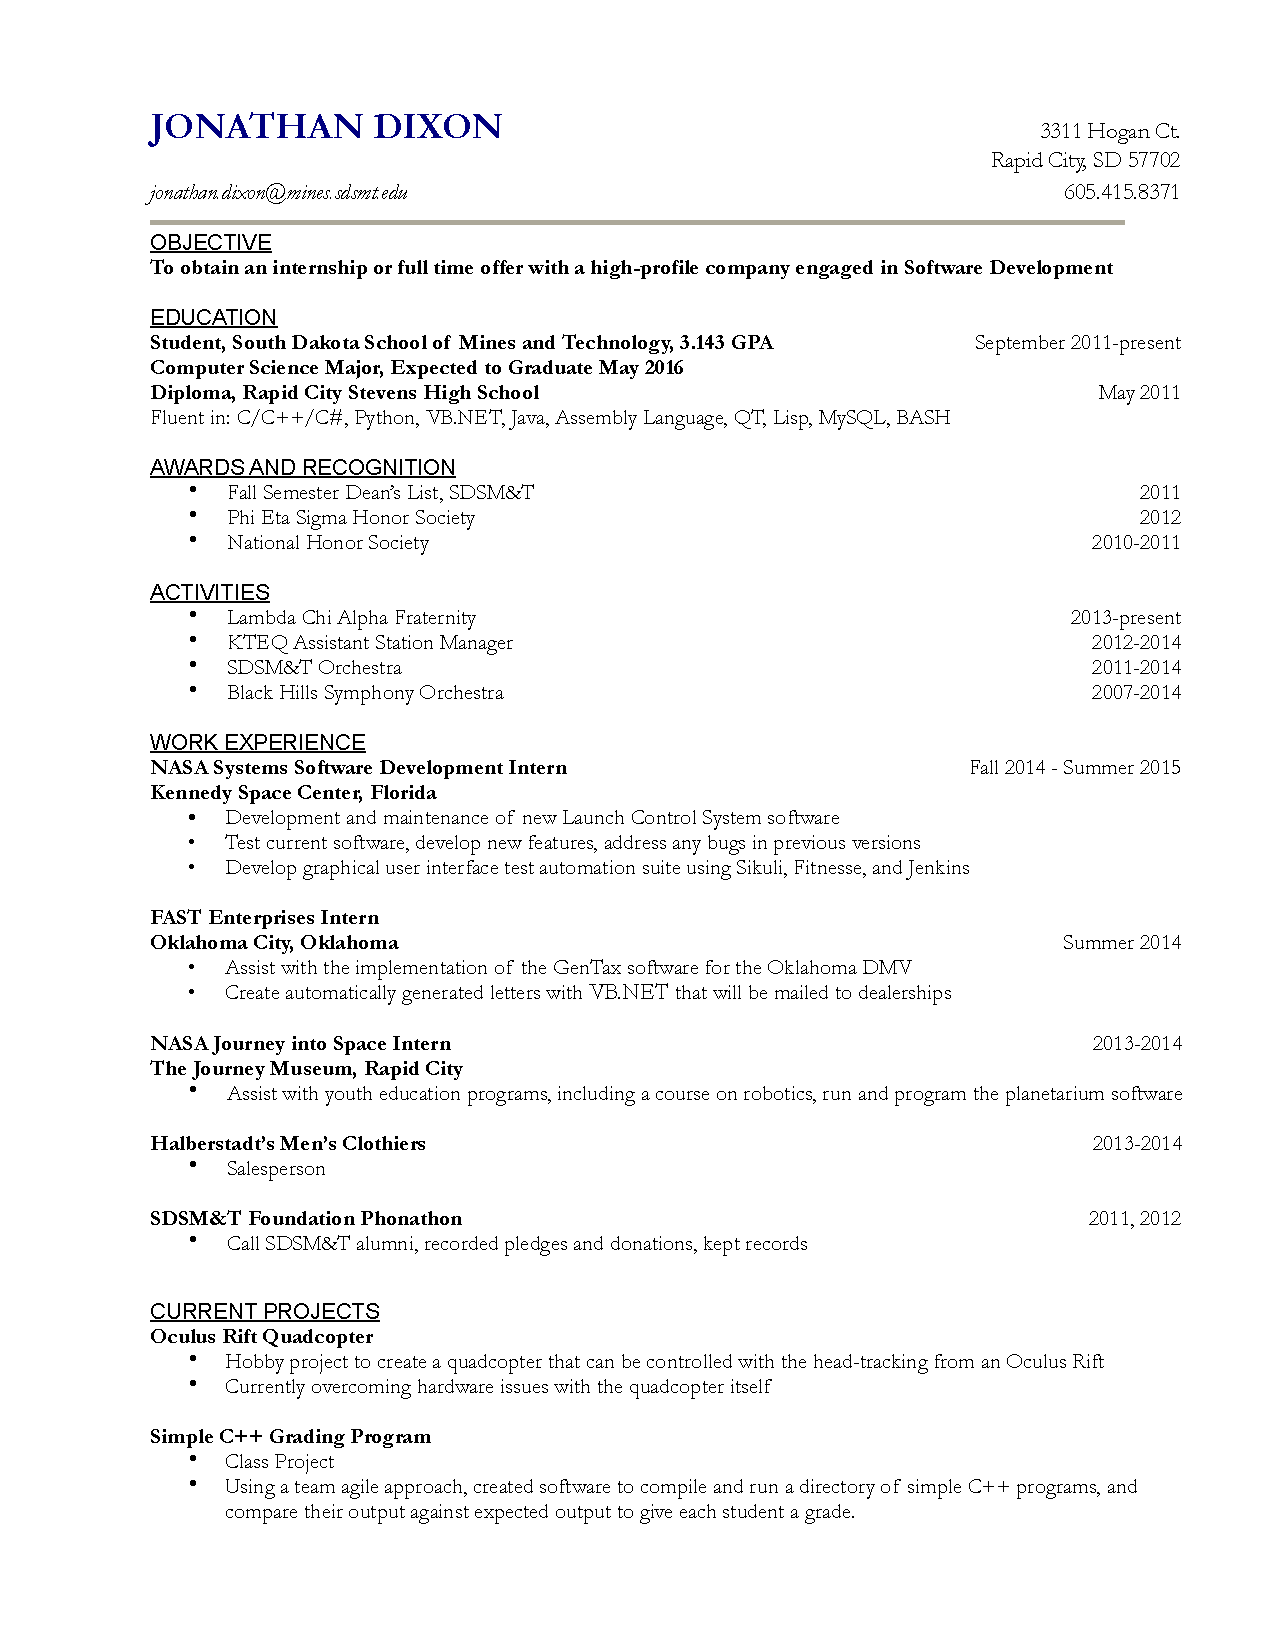
\includepdf{JonathanDixon_Resume_2015.pdf}
     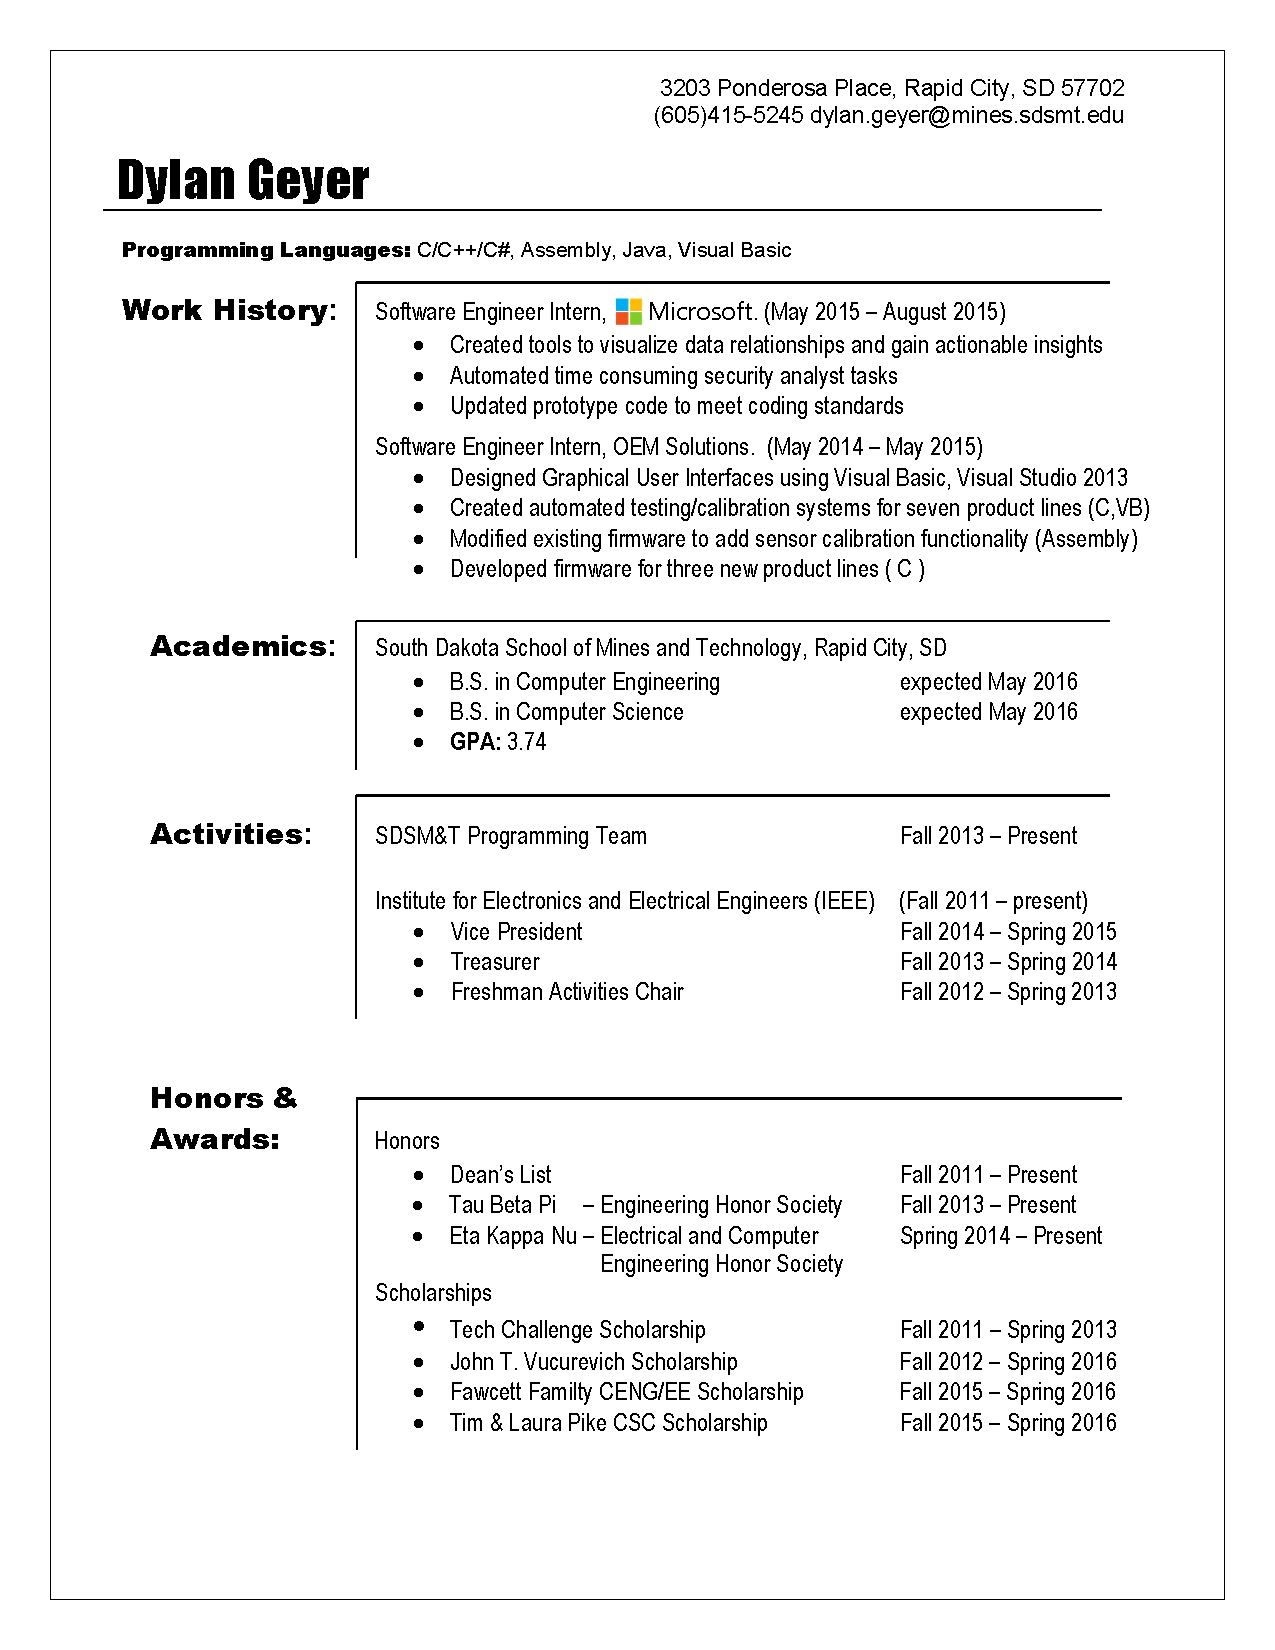
\includepdf{DylanGeyerResume-6-29-2015.pdf}
     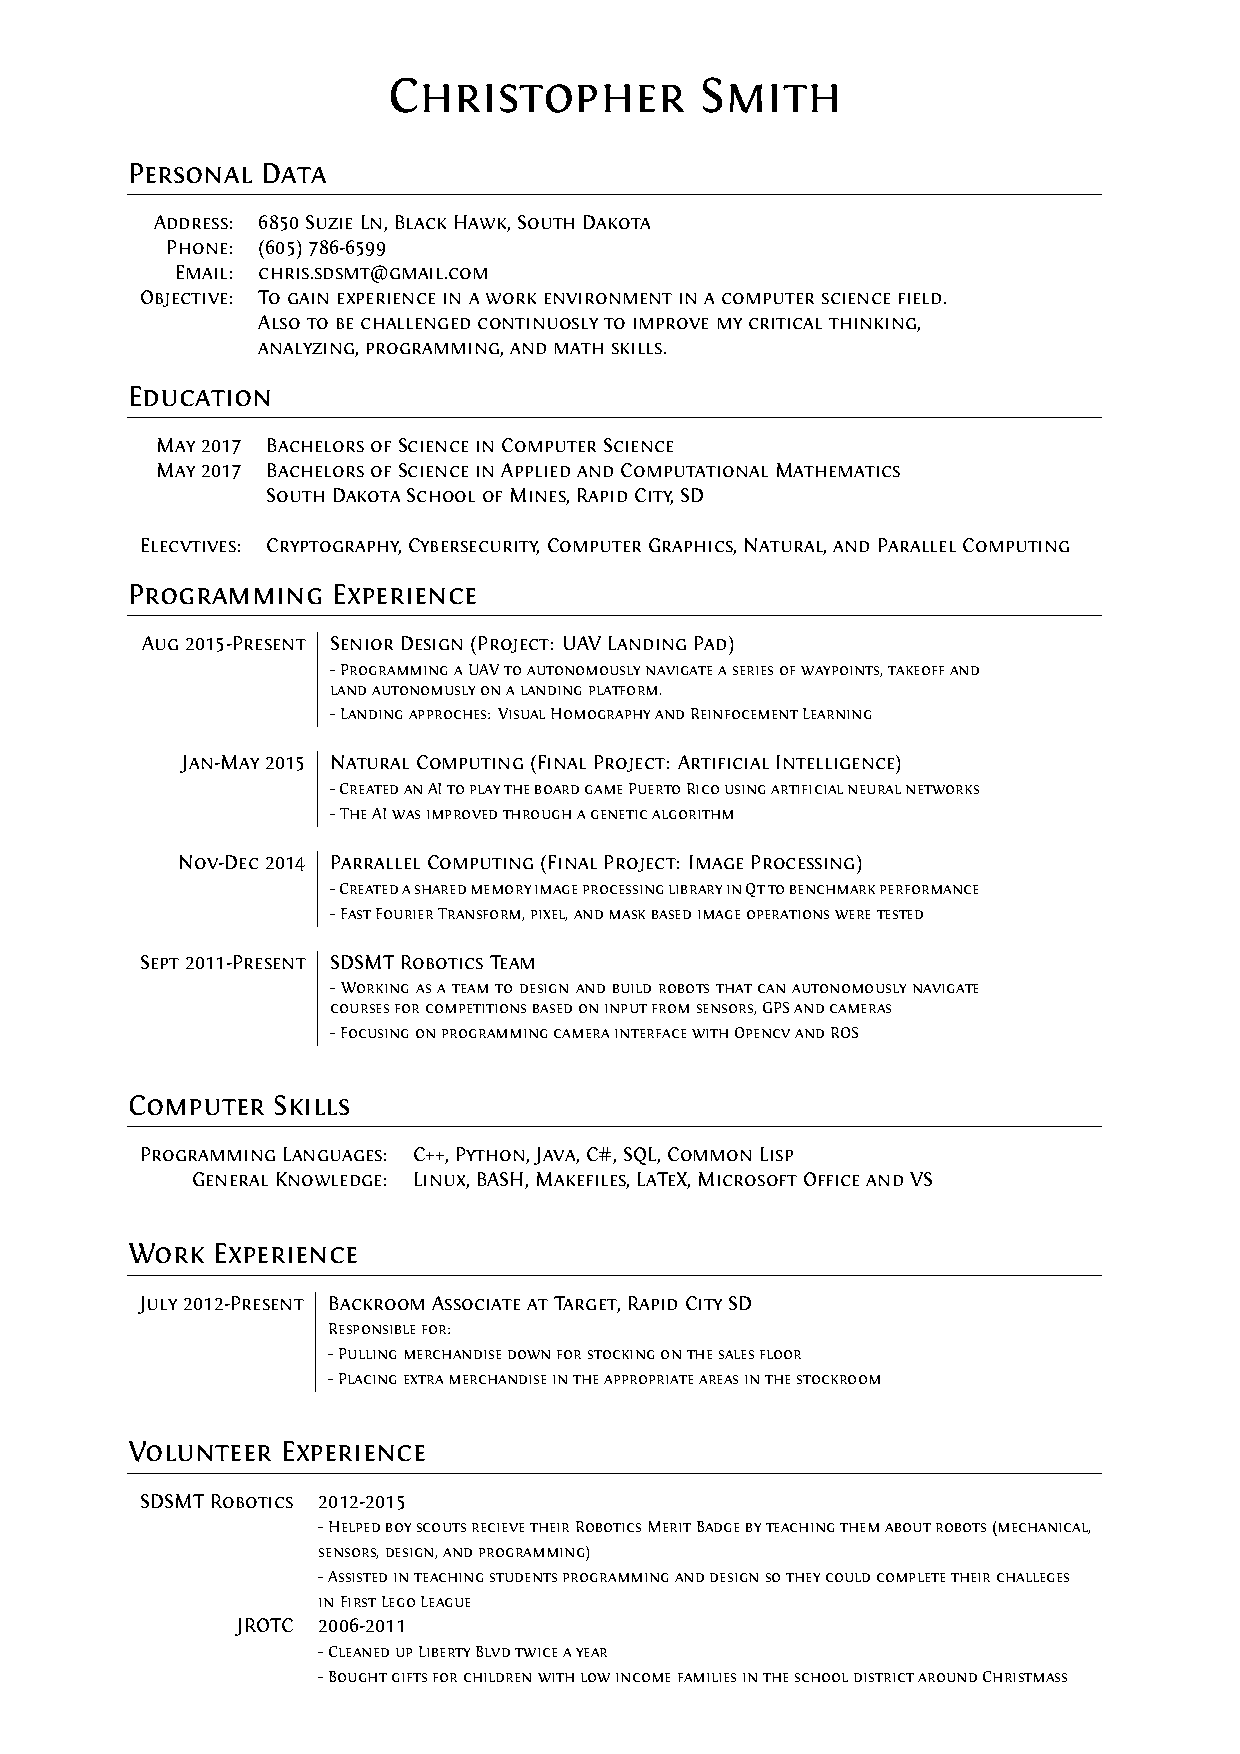
\includepdf{chris_smith_resume.pdf}
     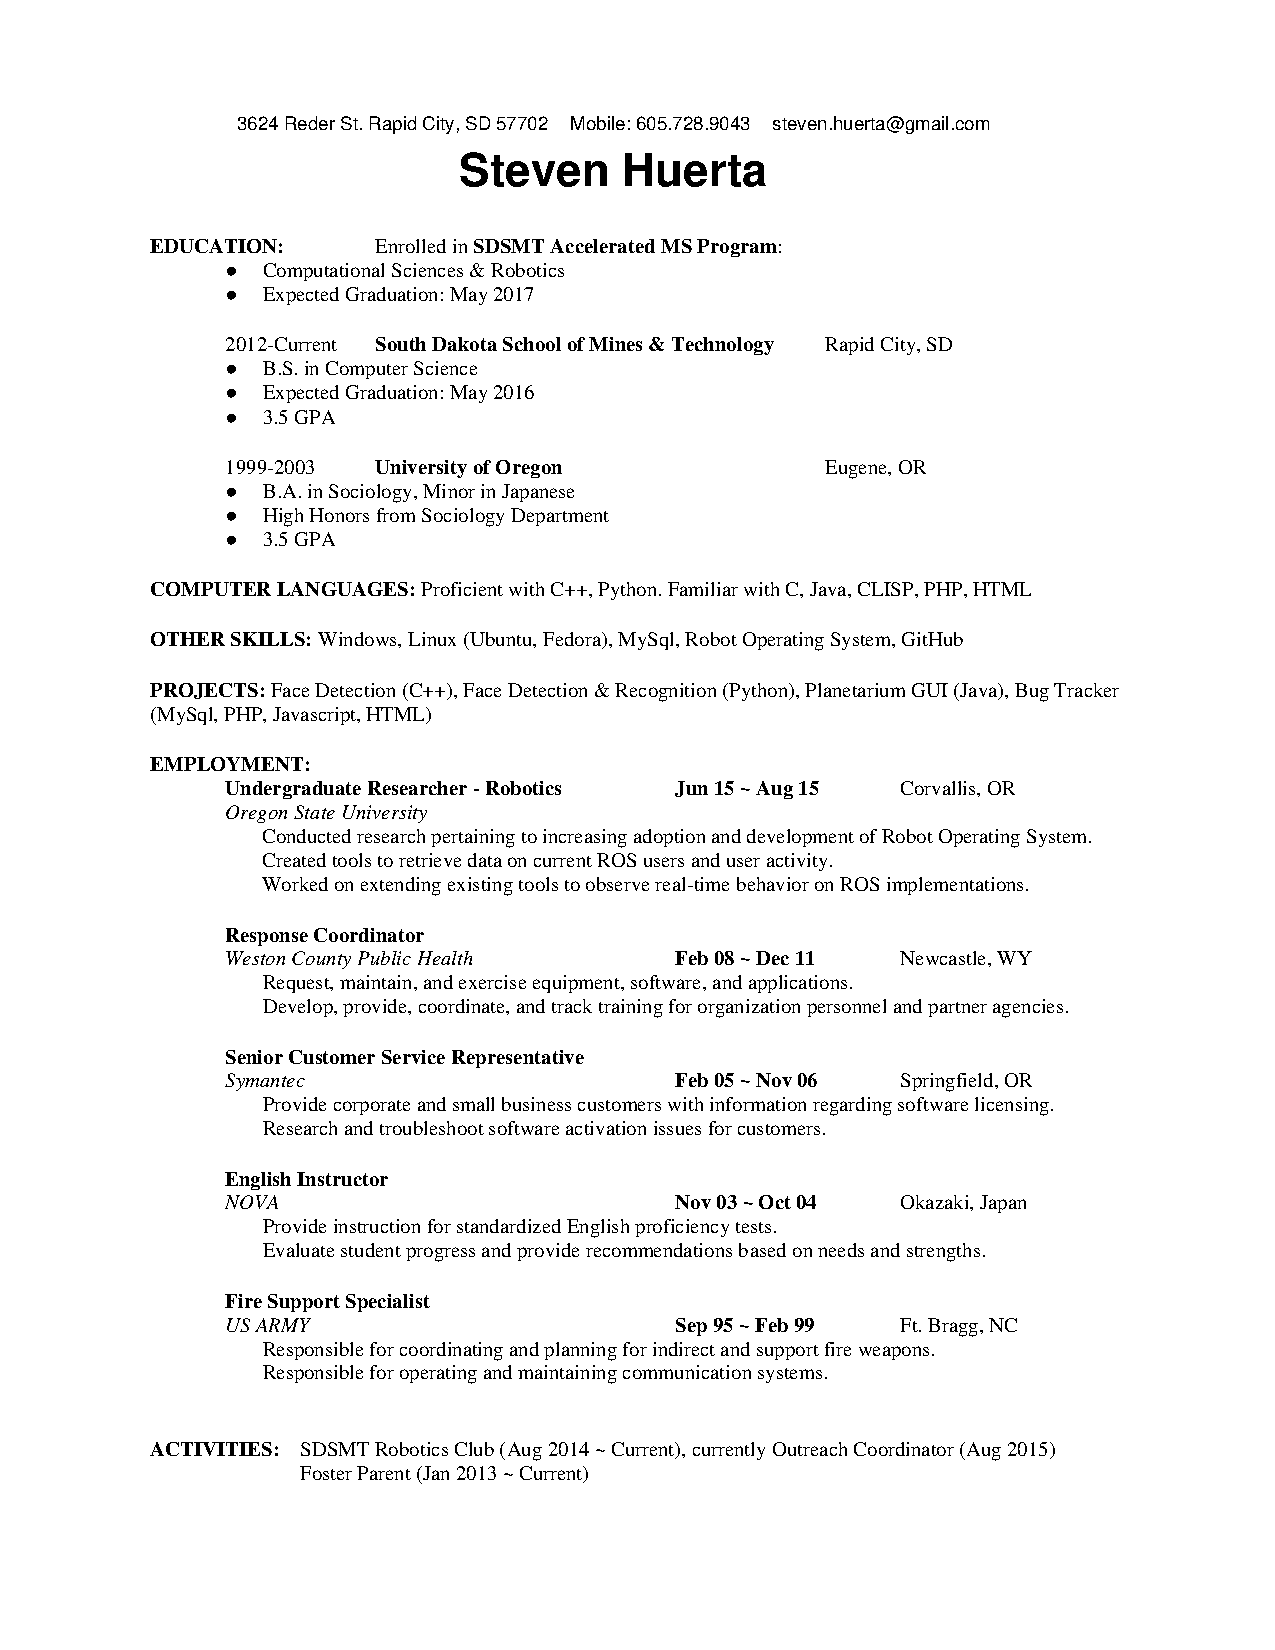
\includepdf{s_huerta_resume.pdf}     

\section{ABET:  Industrial Experience Reports}

\subsection{Jonathan Dixon}

% \includepdf{name1.pdf}

\subsection{Dylan Geyer}
\large{\textbf{Microsoft Internship (May 2015 - Aug 2015)}}
\begin{itemize}
	\item Created tools to visualize data relationships and gain actionable insights.
	\item Automated time consuming security analyst tasks.
	\item Updated prototype code to meet coding standards.
\end{itemize}

\arge{\textbf{OEM Solutions Internship (May 2014 - Current)}}
\begin{itemize}
	\item Used Visual Basic and .NET framework to interface PC with embedded controllers.
	\item Created automated testing/calibration systems for seven different heat controllers.
	\item Added features to existing heat controller firmware (Assembly).
	\item Wrote firmware for three new heater controllers (C).
\end{itemize}
% \includepdf{name2.pdf}

\subsection{Christopher Smith}

% \includepdf{name3.pdf}

\subsection{Steven Huerta}
--No Industrial Experience--
